%===================================================================%
%                  VIETNAM.TEX                                      %
%===================================================================%

\documentclass{thesissummary}
\hfuzz=5.002pt
\hbadness = 100000


\bibliographystyle{unsrt}    
%\bibliographystyle{numeric}    
% for BibTeX - sorted numerical labels by order of
% first citation.

% A useful Journal macro
\def\Journal#1#2#3#4{{#1} {\bf #2}, #3 (#4)}

% Some useful journal names
\def\NCA{\em Nuovo Cimento}
\def\NIM{\em Nucl. Instrum. Methods}
\def\NIMA{{\em Nucl. Instrum. Methods} A}
\def\NPB{{\em Nucl. Phys.} B}
\def\PLB{{\em Phys. Lett.}  B}
\def\PRL{\em Phys. Rev. Lett.}
\def\PRD{{\em Phys. Rev.} D}
\def\ZPC{{\em Z. Phys.} C}

% Some other macros used in the sample text
\def\st{\scriptstyle}
\def\sst{\scriptscriptstyle}
\def\mco{\multicolumn}
\def\epp{\epsilon^{\prime}}
\def\vep{\varepsilon}
\def\ra{\rightarrow}
\def\ppg{\pi^+\pi^-\gamma}
\def\vp{{\bf p}}
\def\ko{K^0}
\def\kb{\bar{K^0}}
\def\al{\alpha}
\def\ab{\bar{\alpha}}
\def\be{\begin{equation}}
\def\ee{\end{equation}}
\def\bea{\begin{eqnarray}}
\def\eea{\end{eqnarray}}
\def\CPbar{\hbox{{\rm CP}\hskip-1.80em{/}}}
%\def\pt{\ensuremath{p_{\mathrm{T}}}\xspace}
%\def\mjj{\ensuremath{m_{jj}}\xspace}

\newcommand*{\mjj}{\ensuremath{m_{\text{jj}}}\xspace}
\newcommand*{\Ngapjets}{\ensuremath{N^{\text{gap}}_{\text{jets}}}\xspace}
\newcommand*{\ngapjets}{\ensuremath{N^{\text{gap}}_{\text{jets}}}\xspace}
\newcommand*{\Ngapjet}{\ensuremath{N^{\text{gap}}_{\text{jets}}}\xspace}
\newcommand*{\ngapjet}{\ensuremath{N^{\text{gap}}_{\text{jets}}}\xspace}
\newcommand*{\nbins}{\ensuremath{N_{\text{bins}}}\xspace}
\newcommand*{\Nbins}{\ensuremath{N_{\text{bins}}}\xspace}
\newcommand*{\nbin}{\ensuremath{N_{\text{bins}}}\xspace}
\newcommand*{\Nbin}{\ensuremath{N_{\text{bins}}}\xspace}
\newcommand*{\bl}{\ensuremath{b_{\text{L},i}}\xspace}
\newcommand*{\bi}{\ensuremath{b_{i}}\xspace}
\newcommand*{\bL}{\ensuremath{b_{\text{L},i}}\xspace}
\newcommand*{\bh}{\ensuremath{b_{\text{H},i}}\xspace}
\newcommand*{\bH}{\ensuremath{b_{\text{H},i}}\xspace}
\newcommand*{\fx}{\ensuremath{f(x_i)}\xspace}
\newcommand*{\rij}{\ensuremath{\mathcal{R}_{ij}}\xspace}
\newcommand*{\muew}{\ensuremath{\mu_{\text{EW},i}}\xspace}
\newcommand*{\ptjj}{\ensuremath{p_{\text{T},jj}}\xspace}
\newcommand*{\dyjj}{\ensuremath{\Delta y(j,j)}\xspace}
\newcommand*{\pt}{\ensuremath{p_{\text{T}}}\xspace}
\newcommand*{\ptref}{\ensuremath{p_{\text{T}}^{\text{Ref}}}\xspace}
\newcommand*{\ptbal}{\ensuremath{p_{\text{T}}^{\text{Bal}}}\xspace}
\newcommand*{\ptz}{\ensuremath{p_{\text{T}}^Z}\xspace}
\newcommand*{\new}{\ensuremath{N_{\text{EW}}^{\text{Nom}}}\xspace}
\newcommand*{\ptJ}{\ensuremath{p_{\text{T}}^J}\xspace}
\newcommand*{\ptj}{\ensuremath{p_{\text{T}}^j}\xspace}
\newcommand*{\et}{\ensuremath{E_{\text{T}}}\xspace}
\newcommand*{\kt}{\ensuremath{k_{t}}\xspace}
\newcommand*{\jfakee}{\ensuremath{j\rightarrow\!e}\xspace}
\newcommand*{\jfakemu}{\ensuremath{j\rightarrow\mu}\xspace}
\newcommand*{\jfakey}{\ensuremath{j\rightarrow\gamma}\xspace}
\newcommand*{\efakey}{\ensuremath{e\rightarrow\gamma}\xspace}
\newcommand*{\rdb}{\ensuremath{R_{\text{DB}}}\xspace}
\newcommand*{\infb}{\ensuremath{\hspace{2pt}\text{fb}^{-1}}\xspace}
\newcommand*{\dphisigned}{\ensuremath{\Delta\phi_{jj}^{\text{signed}}}\xspace}
\newcommand*{\TeV}{\ensuremath{\hspace{2pt}\text{Te\kern -0.1em V}}\xspace}
\newcommand*{\GeV}{\ensuremath{\hspace{2pt}\text{Ge\kern -0.1em V}}\xspace}
\newcommand*{\MeV}{\ensuremath{\hspace{2pt}\text{Me\kern -0.1em V}}\xspace}
\newcommand*{\microns}{\ensuremath{\mu\text{m}}\xspace}
\newcommand*{\mm}{\ensuremath{\text{mm}}\xspace}
\newcommand*{\lag}{\ensuremath{\mathcal{L}}\xspace}
\newcommand*{\fmunu}{\ensuremath{F_{\mu\nu}}\xspace}
\newcommand*{\dmu}{\ensuremath{\partial_\mu}\xspace}
\newcommand*{\dnu}{\ensuremath{\partial_\nu}\xspace}
\newcommand*{\amu}{\ensuremath{A_\mu}\xspace}
\newcommand*{\anu}{\ensuremath{A_\nu}\xspace}
\newcommand*{\ddmu}{\ensuremath{\partial_\mu\partial^\mu}\xspace}
\newcommand*{\ddnu}{\ensuremath{\partial_\nu\partial^\nu}\xspace}
\newcommand*{\xmu}{\ensuremath{x^\mu}\xspace}
\newcommand*{\xnu}{\ensuremath{x^\nu}\xspace}
\newcommand*{\muf}{\ensuremath{\mu_\text{F}}\xspace}
\newcommand*{\mur}{\ensuremath{\mu_\text{R}}\xspace}
\newcommand*{\alphas}{\ensuremath{\alpha_\text{s}}\xspace}
\newcommand*{\invfb}{\ensuremath{\text{fb}^{-1}}\xspace}
\newcommand*{\microseconds}{\ensuremath{\mu\text{s}}\xspace}
\newcommand*{\MET}{\ensuremath{E_{\text{T}}^{\text{miss}}}\xspace}
\newcommand*{\met}{\ensuremath{E_{\text{T}}^{\text{miss}}}\xspace}
\newcommand*{\ptmiss}{\ensuremath{\mathbf{p}_{\text{T}}^{\text{miss}}}\xspace}
\newcommand*{\zjets}{\ensuremath{Z\text{+jets}}\xspace}
\newcommand*{\zjet}{\ensuremath{Z\text{+jet}}\xspace}
\newcommand*{\zee}{\ensuremath{Z\rightarrow\!e^+e^-}\xspace}
\newcommand*{\zmm}{\ensuremath{Z\rightarrow\mu^+\mu^-}\xspace}
\newcommand*{\zeejets}{\ensuremath{Z(\rightarrow\!e^+e^-)\text{+jets}}\xspace}
\newcommand*{\zeejet}{\ensuremath{Z(\rightarrow\!e^+e^-)\text{+jets}}\xspace}
\newcommand*{\zmmjets}{\ensuremath{Z(\rightarrow\mu\mu)\text{+jets}}\xspace}
\newcommand*{\zmmjet}{\ensuremath{Z(\rightarrow\mu\mu)\text{+jets}}\xspace}
\newcommand*{\yjets}{\ensuremath{\gamma\text{+jets}}\xspace}
\newcommand*{\yjet}{\ensuremath{\gamma\text{+jets}}\xspace}
\newcommand*{\gamjets}{\ensuremath{\gamma\text{+jets}}\xspace}
\newcommand*{\gamjet}{\ensuremath{\gamma\text{+jets}}\xspace}
\newcommand*{\DeltaR}{\ensuremath{\Delta R}\xspace} 
\newcommand*{\zcut}{\ensuremath{z_{\text{cut}}}\xspace}
\newcommand*{\Rcut}{\ensuremath{R_{\text{cut}}}\xspace}
\newcommand*{\fcut}{\ensuremath{f_{\text{cut}}}\xspace}
\newcommand*{\Rsub}{\ensuremath{R_{\text{sub}}}\xspace}
\newcommand*{\tu}{\textunderscore}

\newcommand*{\jjpt}{\ensuremath{p_{\text{T}}^{\text{jj}}}\xspace}
\newcommand*{\jjdphi}{\ensuremath{\Delta\phi_{\text{jj}}^{\text{signed}}}\xspace}
\newcommand*{\lepgam}{\ensuremath{\Delta\phi_{\ell\gamma}^{\text{signed}}}\xspace}
\newcommand*{\lepgamdphi}{\ensuremath{\Delta\phi_{\ell\gamma}^{\text{signed}}}\xspace}
\newcommand*{\ptlep}{\ensuremath{p_{\text{T}}^{\ell}}\xspace}
\newcommand*{\leppt}{\ensuremath{p_{\text{T}}^{\ell}}\xspace}
\newcommand*{\wym}{\ensuremath{m_{\ell\gamma}}\xspace}
\newcommand*{\mwy}{\ensuremath{m_{\ell\gamma}}\xspace}
\newcommand*{\lym}{\ensuremath{m_{\ell\gamma}}\xspace}
\newcommand*{\mly}{\ensuremath{m_{\ell\gamma}}\xspace}
\newcommand*{\xiwy}{\ensuremath{\xi_{W\gamma}}}
\newcommand*{\xiwytruth}{\ensuremath{\xi_{W\gamma}^{\text{truth}}}}
\newcommand*{\xiwyreco}{\ensuremath{\xi_{W\gamma}^{\text{reco}}}}
\newcommand*{\xily}{\ensuremath{\xi_{l\gamma}}}
\newcommand*{\lyxi}{\ensuremath{\xi_{l\gamma}}}
\newcommand*{\xilytruth}{\ensuremath{\xi_{l\gamma}^{\text{truth}}}}
\newcommand*{\xilyreco}{\ensuremath{\xi_{l\gamma}^{\text{reco}}}}
\newcommand*{\qcdwy}{\ensuremath{\text{strong-}W\gamma\text{jj }}}
\newcommand*{\Qcdwy}{\ensuremath{\text{Strong-}W\gamma\text{jj }}}
\newcommand*{\ewwy}{\ensuremath{\text{EW-}W\gamma\text{jj }}}
\newcommand*{\Ewwy}{\ensuremath{\text{EW-}W\gamma\text{jj }}}
\newcommand*{\wyjj}{\ensuremath{W\gamma\text{jj }}}

% +--------------------------------------------------------------------+
% |  Monte Carlo generators                                            |
% +--------------------------------------------------------------------+
% Set up generic command for MC with optional version number
%%% e.g. \PYTHIA[8] -> Pythia 8
\NewDocumentCommand {\AtlasMC} { o m } {%
  \IfNoValueTF {#1} {%
    \textsc{#2}\xspace%
  }{%
    \textsc{#2}\,#1\xspace%
  }%
}
\NewDocumentCommand {\ACERMC} { o } {\AtlasMC[#1]{AcerMC}}
\NewDocumentCommand {\ALPGEN} { o } {\AtlasMC[#1]{Alpgen}}
\NewDocumentCommand {\AMEGIC} { o } {\AtlasMC[#1]{Amegic}}
\NewDocumentCommand {\AMCatNLO} { o } {\AtlasMC[#1]{aMC@NLO}}
\NewDocumentCommand {\BLACKHAT} { o } {\AtlasMC[#1]{BlackHat}}
\NewDocumentCommand {\CALCHEP} { o } {\AtlasMC[#1]{CalcHEP}}
\NewDocumentCommand {\COLLIER} { o } {\AtlasMC[#1]{Collier}}
\NewDocumentCommand {\COMPHEP} { o } {\AtlasMC[#1]{CompHEP}}
\NewDocumentCommand {\EVTGEN} { o } {\AtlasMC[#1]{EvtGen}}
\NewDocumentCommand {\FEYNRULES} { o } {\AtlasMC[#1]{FeynRules}}
\NewDocumentCommand {\GGTOVV} { o } {\AtlasMC[#1]{gg2VV}}
\NewDocumentCommand {\GOSAM} { o } {\AtlasMC[#1]{GoSam}}
\NewDocumentCommand {\HATHOR} { o } {\AtlasMC[#1]{Hathor}}
\NewDocumentCommand {\Herwig} { o } {\AtlasMC[#1]{Herwig}}
\NewDocumentCommand {\HERWIG} { o } {\AtlasMC[#1]{Herwig}}
\NewDocumentCommand {\HERWIGpp} { o } {\AtlasMC[#1]{Herwig++}}
\NewDocumentCommand {\HRES} { o } {\AtlasMC[#1]{Hres}}
\NewDocumentCommand {\JIMMY} { o } {\AtlasMC[#1]{Jimmy}}
\NewDocumentCommand {\MADSPIN} { o } {\AtlasMC[#1]{MadSpin}}
\NewDocumentCommand {\MADGRAPH} { o } {\AtlasMC[#1]{MadGraph}}
\NewDocumentCommand {\MGNLO} { o } {\AtlasMC[#1]{MadGraph5\_aMC@NLO}} %short-hand
\NewDocumentCommand {\MCatNLO} { o } {\AtlasMC[#1]{MC@NLO}}
\NewDocumentCommand {\MCFM} { o } {\AtlasMC[#1]{MCFM}}
\NewDocumentCommand {\METOP} { o } {\AtlasMC[#1]{METOP}}
\NewDocumentCommand {\OPENLOOPS} { o } {\AtlasMC[#1]{OpenLoops}}
\NewDocumentCommand {\POWHEG} { o } {\AtlasMC[#1]{Powheg}}
\NewDocumentCommand {\POWHEGBOX} { o } {\AtlasMC[#1]{Powheg-Box}}
\NewDocumentCommand {\POWHEGBOXRES} { o } {\AtlasMC[#1]{Powheg\,Box\,Res}}
\NewDocumentCommand {\PHOTOS} { o } {\AtlasMC[#1]{Photos}}
\NewDocumentCommand {\COMIX} { o } {\AtlasMC[#1]{Comix}}
\NewDocumentCommand {\PHOTOSpp} { o } {\AtlasMC[#1]{Photos++}}
\NewDocumentCommand {\PROPHECY} { o } {\AtlasMC[#1]{Prophecy4f}}
\NewDocumentCommand {\PROTOS} { o } {\AtlasMC[#1]{Protos}}
\NewDocumentCommand {\CSShower} { o } {\AtlasMC[#1]{CSShower}}
\NewDocumentCommand {\Pythia} { o } {\AtlasMC[#1]{Pythia8}}
\NewDocumentCommand {\PYTHIA} { o } {\AtlasMC[#1]{Pythia8}}
\NewDocumentCommand {\RECOLA} { o } {\AtlasMC[#1]{Recola}}
\NewDocumentCommand {\Sherpa} { o } {\AtlasMC[#1]{Sherpa}}
\NewDocumentCommand {\SHERPA} { o } {\AtlasMC[#1]{Sherpa}}
\NewDocumentCommand {\Fastjet} { o } {\AtlasMC[#1]{FastJet}}
\NewDocumentCommand {\FastJet} { o } {\AtlasMC[#1]{FastJet}}
\NewDocumentCommand {\FASTJET} { o } {\AtlasMC[#1]{FastJet}}
\NewDocumentCommand {\TOPpp} { o } {\AtlasMC[#1]{Top++}}
\NewDocumentCommand {\VBFNLO} { o } {\AtlasMC[#1]{VBFNLO}}

% common ME+PS combinations
\NewDocumentCommand {\MGNLOHER} { o } {\AtlasMC[#1]{MadGraph5\_aMC@NLO+Herwig}}
\NewDocumentCommand {\MGNLOPY} { o } {\AtlasMC[#1]{MadGraph5\_aMC@NLO+Pythia}}
\NewDocumentCommand {\MGHER} { o } {\AtlasMC[#1]{MadGraph5+Herwig}}
\NewDocumentCommand {\MGPY} { o } {\AtlasMC[#1]{MadGraph5+Pythia}}
\NewDocumentCommand {\POWHER} { o } {\AtlasMC[#1]{Powheg+Herwig}}
\NewDocumentCommand {\POWPY} { o } {\AtlasMC[#1]{Powheg+Pythia}}
\NewDocumentCommand {\SHERPABH} { o } {\AtlasMC[#1]{Sherpa+BlackHat}}
\NewDocumentCommand {\SHERPAOL} { o } {\AtlasMC[#1]{Sherpa+OpenLoops}}


%%% Set up generic command for common PDFs with optional 
%%% version number/perturbative order (but no space)
%%% e.g. \NNPDF[3.0nnlo] -> NNPDF3.0nnlo
\NewDocumentCommand {\AtlasPDF} { o m } {%
  \IfNoValueTF {#1} {%
    \textsc{#2}\xspace%
  }{%
    \textsc{#2#1}\xspace%
  }%
}
\NewDocumentCommand {\ABM} { o } {\AtlasPDF[#1]{ABM}}
\NewDocumentCommand {\ABKM} { o } {\AtlasPDF[#1]{ABKM}}
\NewDocumentCommand {\CT} { o } {\AtlasPDF[#1]{CT}}
\NewDocumentCommand {\CTEQ} { o } {\AtlasPDF[#1]{CTEQ}}
\NewDocumentCommand {\GJR} { o } {\AtlasPDF[#1]{GJR}}
\NewDocumentCommand {\HERAPDF} { o } {\AtlasPDF[#1]{HERAPDF}}
\NewDocumentCommand {\LUXQED} { o } {\AtlasPDF[#1]{LUXqed}}
\NewDocumentCommand {\MSTW} { o } {\AtlasPDF[#1]{MSTW2008}}
\NewDocumentCommand {\MMHT} { o } {\AtlasPDF[#1]{MMHT2014}}
\NewDocumentCommand {\MSHT} { o } {\AtlasPDF[#1]{MSHT2020}}
\NewDocumentCommand {\NNPDF} { o } {\AtlasPDF[#1]{NNPDF3.0nnlo}}
\NewDocumentCommand {\NNPDFlo} { o } {\AtlasPDF[#1]{NNPDF3.1lo}}
\NewDocumentCommand {\NNPDFtwolo} { o } {\AtlasPDF[#1]{NNPDF2.3lo}}
\NewDocumentCommand {\NNPDFnlo} { o } {\AtlasPDF[#1]{NNPDF3.0nlo}}
\NewDocumentCommand {\PDFforLHC} { o } {\AtlasPDF[#1]{PDF4LHC}}

%%% Event generator extras
\newcommand*{\AUET}{AUET2\xspace}
\newcommand*{\AZNLO}{AZNLO\xspace}
\newcommand*{\FXFX}{\textsc{FxFx}\xspace}
\newcommand*{\GEANT}{\textsc{Geant4}\xspace}
\newcommand*{\MENLOPS}{\textsc{MENLOPS}\xspace}
\newcommand*{\MEPSatLO}{\textsc{MEPS@LO}\xspace}
\newcommand*{\MEPSatNLO}{\textsc{MEPS@NLO}\xspace}
\newcommand*{\MINLO}{\textsc{MiNLO}\xspace}
\newcommand*{\Monash}{Monash\xspace}
\newcommand*{\Perugia}{Perugia\xspace}
\newcommand*{\Prospino}{Prospino\xspace}
\newcommand*{\UEEE}{UE-EE-5\xspace}

\newcommand*{\LO}{\ensuremath{\text{LO}}\xspace}
\newcommand*{\NLO}{\ensuremath{\text{NLO}}\xspace}
\newcommand*{\NLL}{\ensuremath{\text{NLL}}\xspace}
\newcommand*{\NNLO}{\ensuremath{\text{N}}\NLO}
\newcommand*{\muF}{\ensuremath{\mu_\mathrm{f}}\xspace}
\newcommand*{\muQ}{\ensuremath{\mu_\mathrm{q}}\xspace}
\newcommand*{\muR}{\ensuremath{\mu_\mathrm{r}}\xspace}
\newcommand*{\hdamp}{\ensuremath{h_\mathrm{damp}}\xspace}
\newcommand*{\NLOEWvirt}{NLO~\ensuremath{\text{EW}_\text{virt}}\xspace}


\usepackage{tabularx,ragged2e,xspace,placeins,amstext,siunitx,caption,subcaption,multirow,booktabs,float,amsmath,amssymb,mathtools,cleveref,slashed,dsfont,stackengine,mathrsfs,tikz,lineno}
\usepackage[inline]{enumitem}
%\usepackage[style=numeric]{biblatex}
\linenumbers
%temp replacement due to no font
%%%%%%%%%%%%%%%%%%%%%%%%%%%%%%%%%%%%%%%%%%%%%%%%%%
%                                                %
%    BEGINNING OF TEXT                           %
%                                                %
%%%%%%%%%%%%%%%%%%%%%%%%%%%%%%%%%%%%%%%%%%%%%%%%%%

%\newcommand{\Photo}{
\includegraphics[height=35mm]{figures/me2.jpg}}
%\newcommand{\Photo}{}
%
\begin{document}
%\vspace*{4cm}
\title{In-situ Jet Calibration and Electro-Weak Induced Production of W$\gamma$ in Association With Two Jets at ATLAS}

\author{ Benjamin Honan }

\address{School of Physics and Astronomy, University of Manchester, M13 9PL, United Kingdom}
\maketitle
\strut\newline
\noindent
The submitted thesis presents original work pertaining to differential cross-section measurements of \wyjj production in the electro-weak (EW) production mode (no strong coupling vertices at leading order), in addition to the derivation of in-situ corrections to the jet energy scale (JES) for large-radius jets\footnote{A large radius jet is reconstructed using an anti-\kt ``$R$'' parameter of $R=1.0$, which is useful where there are highly collimated decay products originating from high-\pt massive particles.}, which was performed as the author's qualification task.

\section{In-situ Calibration of Large-R Jets}

The JES is a numerical factor that corrects the measured energy of reconstructed jets to that of simulated truth particles. Before the JES can be applied to data, a residual correction is calculated using data-to-simulation ratios primarily to account for detector effects not captured by simulation. This is called the \textit{in-situ} calibration. The calibration is performed using \zjet events in both the electron and muon decay channels.
\\\\
In-situ corrections are derived for large-R jets that have been reconstructed using ``unified flow object'' (UFO) input objects. UFOs form the inputs to the anti-\kt jet reconstruction algorithm, and are built using combined calorimeter and track information. UFO jets are designed to have good performance at high and low \pt, and in dense environments by combining the PFlow \cite{pflow} and TCC \cite{tcc} algorithms.
\\\\
The in-situ calibration is derived with the direct balance method using \zjet events, where the \pt of the well-measured dilepton (reference) system is balanced against the \pt of a large-R jet (a so-called $2\rightarrow2$ topology) in the central ($|\eta|<0.8$) region of the detector. The in-situ correction is defined as the double ratio of the response $\mathcal{R}$ in data divided by the response in simulation, where the response is defined as 
\begin{equation}
    \mathcal{R} \equiv \Bigg\langle\frac{\pt^{\text{jet}}}{\pt^{\text{ref}}}\Bigg\rangle \equiv \langle\pt^{\text{bal}}\rangle,
\end{equation},
where $\pt^{\text{ref}}$ is the \pt of the reference system, and $\pt^{\text{jet}}$ is the \pt of the jet being calibrated.
\\\\
The response is sensitive to secondary effects such as QCD radiation outside of the jet cone. Hence, to reduce the model-dependence of the calibration, events are selected such that they have a near $2\rightarrow2$ topology. The response is calculated separately in electron and muon channels as a function of $\pt^{\text{ref}}$ by fitting a Gaussian to the $\pt^{\text{bal}}$ distribution for each bin, and taking the mean from the Gaussian.\footnote{The response is non-Gaussian if measured in $\pt^{\text{jet}}$ bins. A transformation from $\pt^{\text{ref}}$ to $\pt^{\text{jet}}$ is derived for each bin for the final calibration.}
\\\\
In addition to the uncertainty arising from the statistical precision of the data, the calibration is subject to systematic uncertainties which arise from the choice of Monte-Carlo (MC) event generator used for the \zjet sample, lepton scale and resolution effects, the statistical precision of the \zjet sample, and variations in the event selection criteria. All systematic uncertainties are re-binned in $\pt^{\text{ref}}$ such that they are statistically significant at the level of $2\sigma$. The dominant uncertainties are from MC modelling and statistical uncertainties. The total uncertainty on the calibration is below $1\%$ for most bins.
\\\\
The final calibration used by ATLAS analyses is derived by combining the \zjet calibration with the $\gamma+\text{jet}$ and multi-jet calibrations (not performed by the author). The \zjet calibration was observed to be consistent in shape with the $\gamma+\text{jet}$ calibration, and was found to be relevant in the $200-500\GeV$ range.
%repeated using of zjets, make sure \zjet is used rather than \zjets.

\section{Differential Cross-section Measurements of Electro-Weak \wyjj Production}

\Ewwy production is of particular interest because of the sensitivity to vector boson scattering (VBS) interactions. VBS processes are defined by the t-channel exchange of EW bosons (Z,W,$\gamma$) resulting in two EW bosons in the final state. These processes are sensitive to anomalous (zero in the standard model) trilinear (aTGC) and quartic (aQGC) gauge couplings. Precise measurements of VBS-sensitive processes are therefore well suited to the derivation of constraints on aQGCs as these represent the lowest order processes involving quartic interactions between EW bosons. This work contributed to the publication \cite{vbswy}, which also provided the first observation of \ewwy production at ATLAS. 
\\\\
%* Define a VBS-enhanced phasespace through centrality, mjj, rapidity cuts (others?)
%* Extract signal and constrain background simultaneously using minimum log-likelihood fit (SR and CRs)
%* Motivation behind using f(x)=c, including the plots you invented
%* Derivation of systematic uncertainties, bootstrapping
%* Unfolding and final results
%
Unfolded differential cross-sections are measured for six different observables. These are the dijet invariant mass \mjj, dijet transverse momentum \ptjj, signed dijet azimuthal angle separation \jjdphi, lepton transverse momentum \ptlep, signed azimuthal angle separation of the lepton and the photon \lepgamdphi, and the invariant mass of the lepton-photon system \mly. The measurements are performed in a VBS-enriched kinematic region through the large dijet mass requirement ($\mjj>1\TeV$), and through a requirement on the rapidity separation of the tagging jets ($\dyjj>2$). 
Additionally, a signal region (SR) is defined through requirements on the number of jets in the rapidity interval between the tagging jets ($\ngapjet=0$), and on the \textit{centrality} of the lepton-photon system ($\xily<0.35$)
where 
\begin{equation} 
    \xi_{l\gamma}\equiv\frac{|(y_{l\gamma}-(y_{j1}+y_{j2})/2)|}{|(y_{j1}-y_{j2})|},
\end{equation}
and the symbol $y$ represents the rapidity of the leading jet ($j1$), sub-leading jet ($j2$), or the lepton-photon ($\ell\gamma$) system.
Additional object and event selections are applied to reject backgrounds, and to improve the signal purity in the SR. These backgrounds are from \qcdwy production (defined by $W\gamma jj$ production diagrams corresponding to cross-sections of the order of $\alpha_s^2\alpha_{EW}^2$), interference between the strong and EW \wyjj modes, prompt backgrounds from $Z\gamma$ and $tx\gamma$ production, and non-prompt backgrounds arising from mis-reconstructed leptons, photons, or jets. The author was responsible for optimising the SR selection criteria, and contributed to the optimisation of the VBS-enriched region selections.
\\\\
The signal is extracted and the shape and normalisation of the background is constrained simultaneously using a binned minimum log-likelihood fit. The background constraints are derived primarily in regions of low-signal/high-background purity through the definition of three control regions, CRa, CRb, and CRc. These are defined by inverting the \xily and \ngapjet requirements in the definition of the SR. The primary constraint to the strong background is derived in the control region where the \ngapjet cut is inverted (CRa). And a residual correction factor, $c$, is derived primarily in the control region where the centrality cut in inverted (CRc). This factor is designed to correct for non-closure when transferring the background constraint to the SR. The author determined that this transfer factor should purely be an additional normalisation constraint to prevent unstable behaviour in the fit. This was done using a novel method involving correlating pseudo-experiments in individual control regions to their respective effect on the extracted signal yield.
\\\\
The dominant uncertainty on the measurement arises from the statistical precision of the data. The dominant theoretical systematic uncertainty comes from the choice of the \qcdwy sample generator, and the dominant experimental systematic uncertainties correspond to the jet energy scale and jet energy resolution. The author derived all statistical and systematic uncertainties on the extracted signal yields, in addition to the statistical resolution of each source of systematic uncertainty.
\\\\
The final differential cross-sections are derived at particle level by unfolding the differential event yields after extracting the \ewwy signal (the author was responsible for comparing the pre-fit and post-fit unfolded systematic uncertainties). These measurements are compared to predictions from simulations of \ewwy production using the \SHERPA2.2.12 and \MADGRAPH5 event generators at LO accuracy. In general, the results are found to display better agreement with the \SHERPA2.2.12 predictions. These measurements contribute to the derivation of constraints on aQGCs derived through an EFT parametrisation. These results include the first LHC constraints of the $f_{T3}$ and $f_{T4}$ operator couplings. The author provided the yields and systematic breakdowns for each observable for the EFT fit, but was not responsible for performing the fit and the limit-setting.
%$VVjj$ (where $V$ is one of $\gamma,W,Z$) processes occur via the EW and strong associated production modes (and the interference between the two modes). In the EW mode, the jets arise via the EW interaction, and in the strong mode, the jets arise via the strong interaction. An observation and fiducial cross-section measurement of the EW production of opposite-sign WW in association with jets (EW $W^+W^-jj$) is made using the ATLAS detector \cite{osww}. EW $W^+W^-jj$ is sensitive to quartic EW interactions through VBS. The signal region is defined by requiring events to pass: 2-3 jets; an opposite sign electron-muon pair; missing transverse energy $E_\mathrm{T}^{\mathrm{miss}}$ $>$ 15 GeV; and a b-jet veto.
%\begin{itemize}
%       \item 2-3 jets
%       \item An opposite sign electron-muon pair
%       \item $E_\mathrm{T}^{\mathrm{miss}}$ $>$ 15 GeV
%       \item b-jet veto
%\end{itemize}
%In addition, there are requirements on the third lepton, the dilepton centrality and invariant mass, and lepton isolation and ID.  
%A neural network (NN) is trained to distinguish the EW signal from the dominant backgrounds which are the strong production mode of opposite-sign WW, and backgrounds involving top decays. To constrain the dominant background from tops, a top-enriched control region is defined by inverting the b-jet veto requirement. \\\\
%The significance of the observation is determined through a profile-likelihood fit with NN score in the signal and control regions simultaneously. The signal strength, and the strong and top background normalisations are included as floating parameters in the fit. By evaluating the likelihood-ratio test statistic for the background-only hypothesis, EW $W^+W^-jj$ is observed at a significance of $7.1\sigma$. A cross-section of $2.65^{+0.52}_{-0.48}$fb is measured for EW $W^+W^-jj$ in a signal-enriched fiducial volume. The dominant sources of uncertainty are statistical in nature. 

%\begin{figure}
%       \begin{minipage}{6in}
%           \centering
%           \raisebox{-0.5\height}{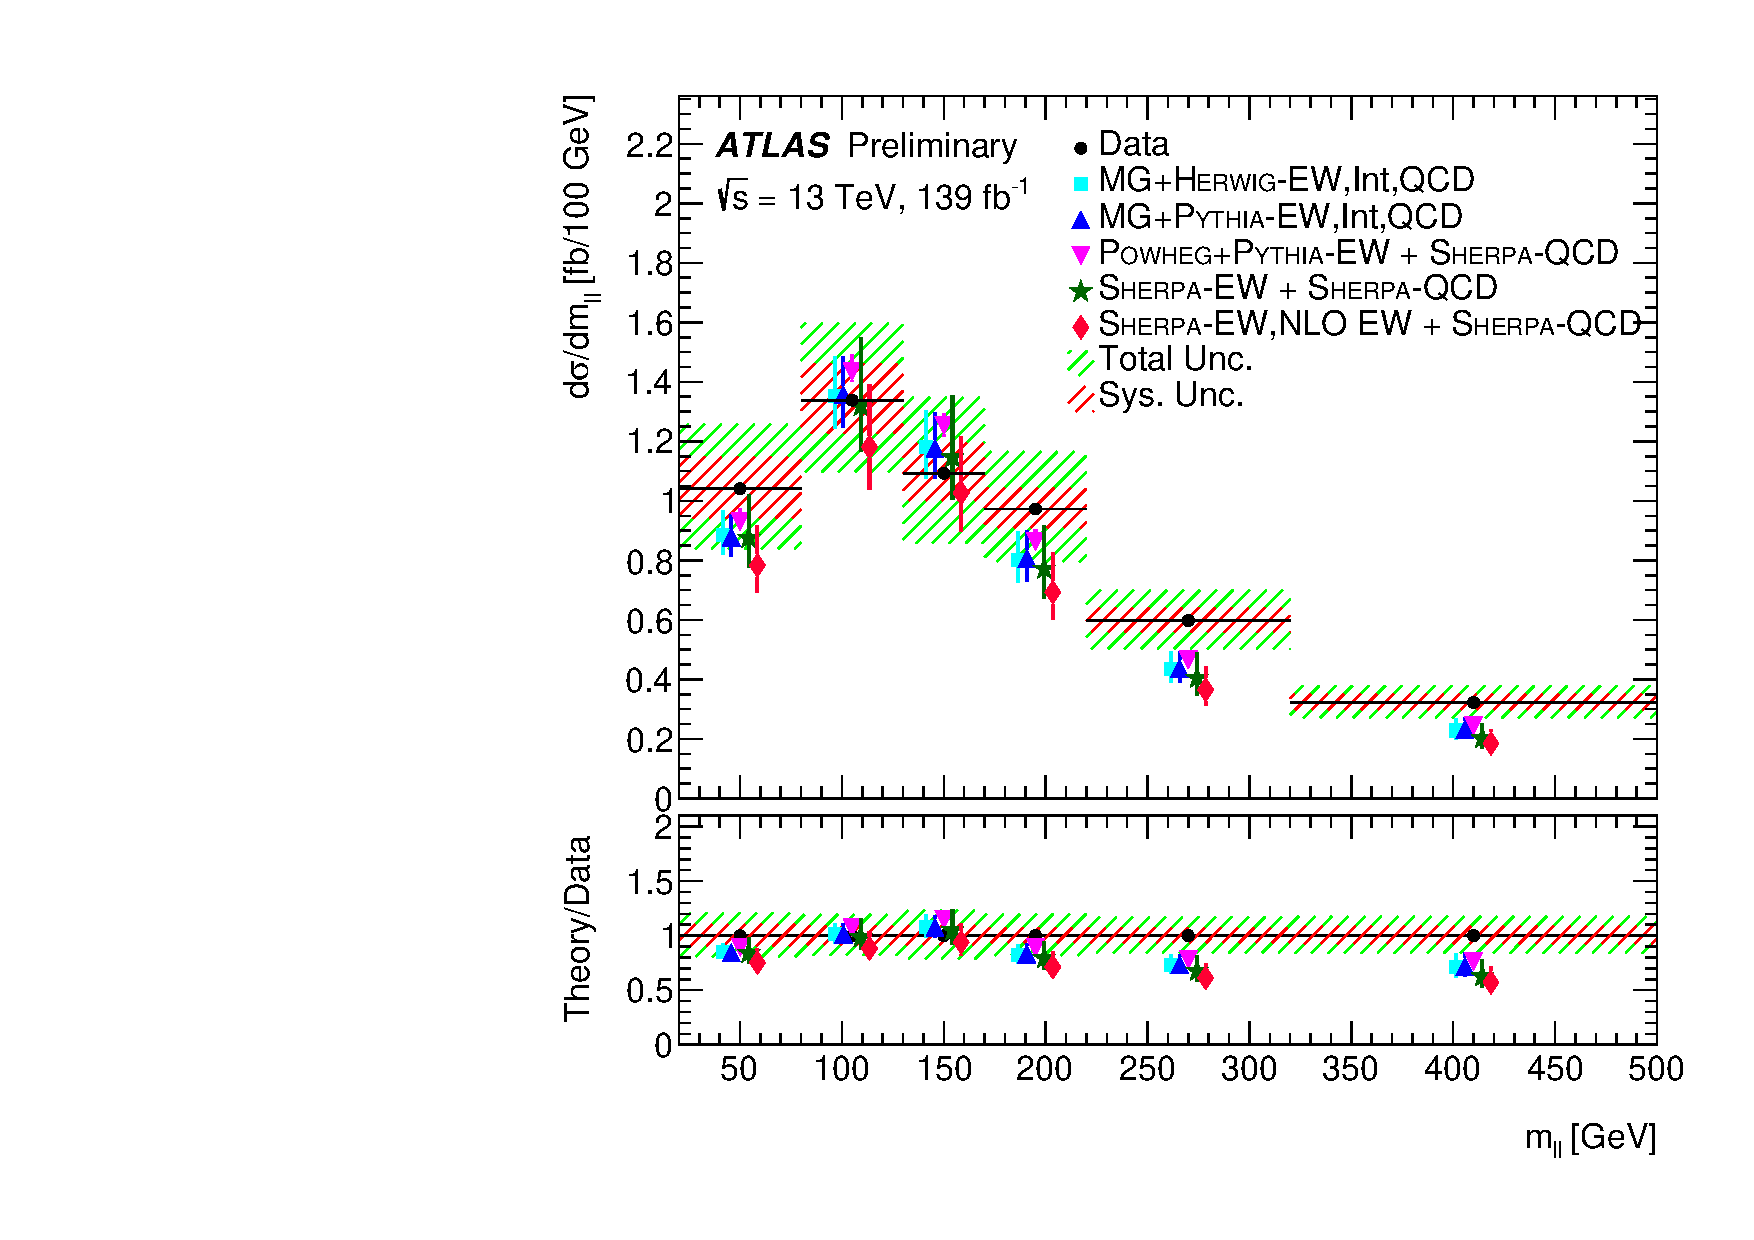
\includegraphics[width=0.49\textwidth]{figures/fig_06a.pdf}}
%           \raisebox{-0.5\height}{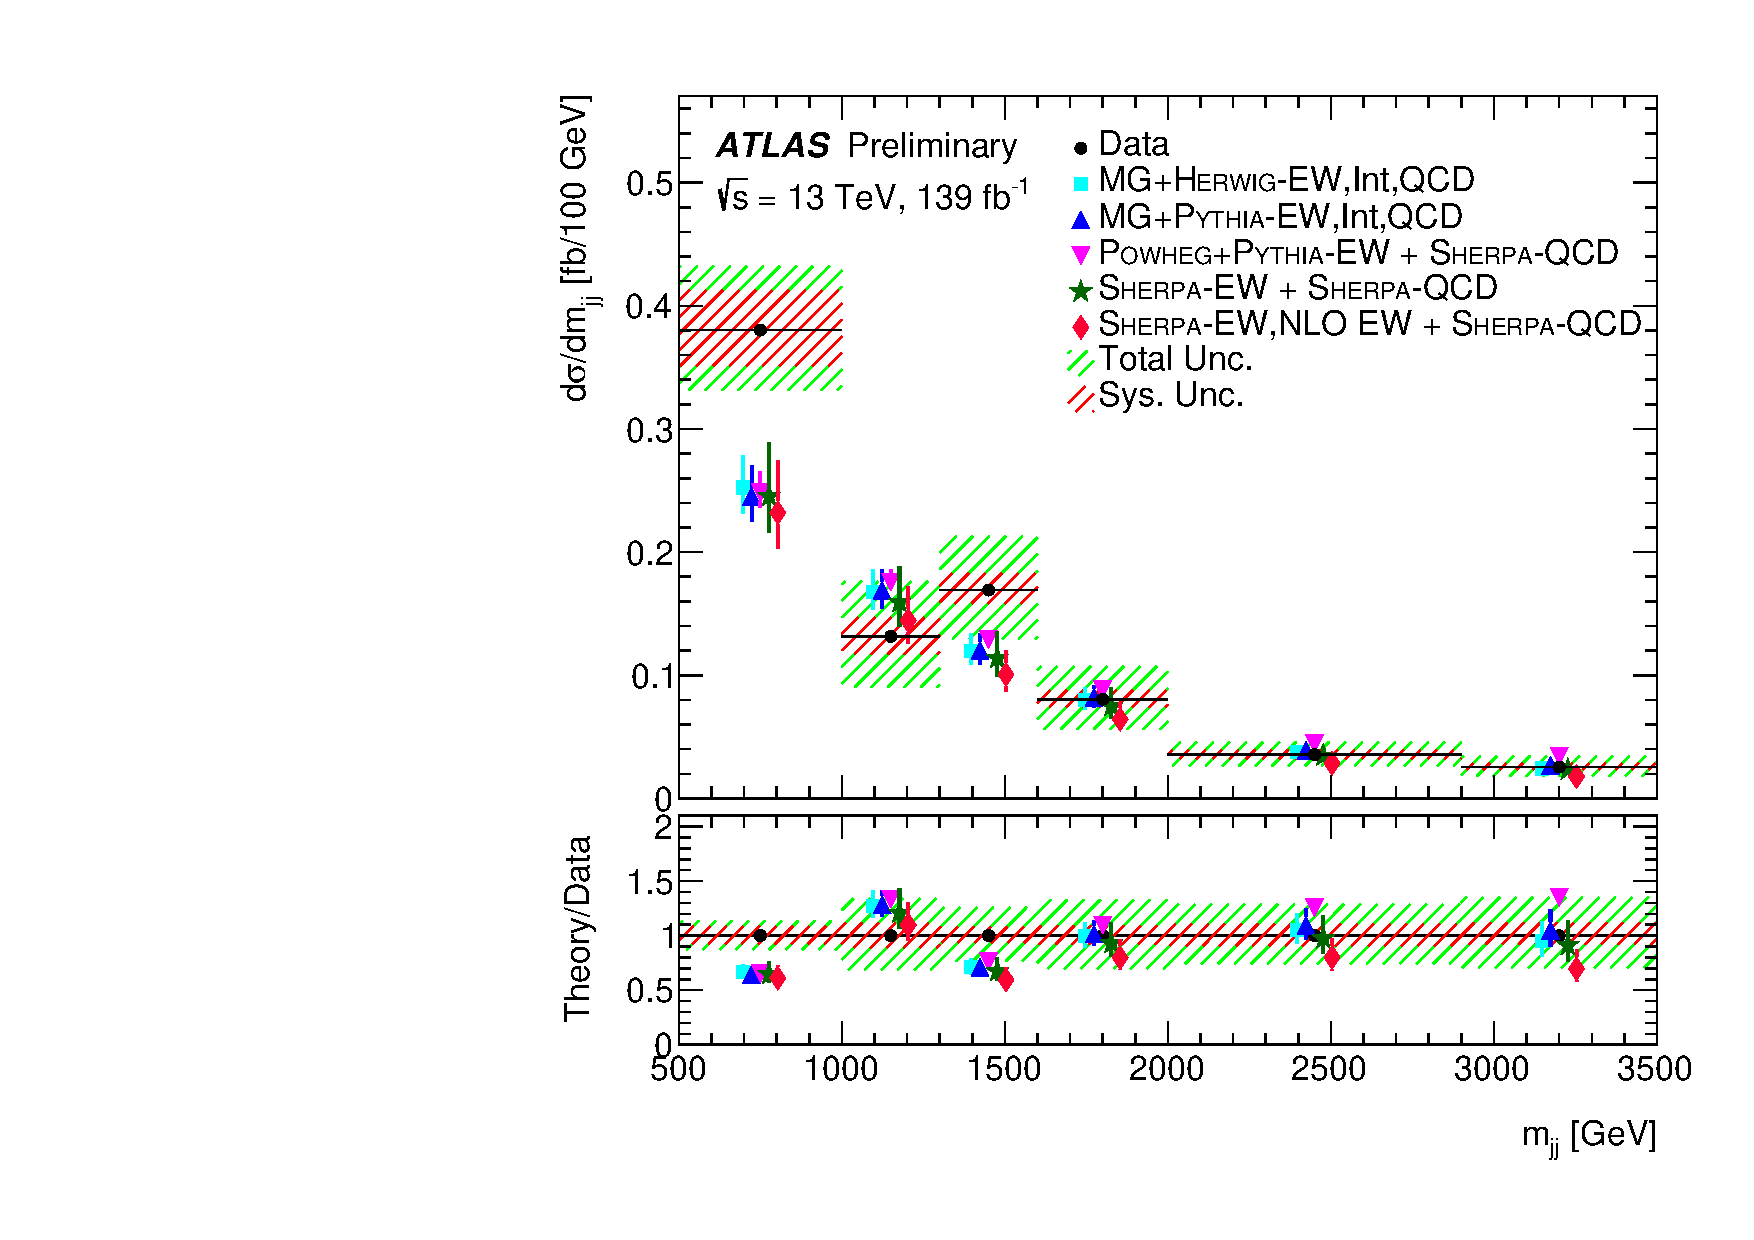
\includegraphics[width=0.49\textwidth]{figures/fig_06c.pdf}}
%           \centering
%       \end{minipage}
%       \caption{Unfolded differential cross-sections of inclusive $W^\pm W^\pm jj$ production with $m_{ll}$ and $m_{jj}$.\protect\cite{ssww}}
%\end{figure}\noindent
%One and two-dimensional limits are set on Wilson coefficients corresponding to dimension-8 (dim-8) EFT operators. Dim-8 is the first time operators appear that only affect the quartic interactions. Since dim $>$ 4 operators can lead to scattering amplitudes that violate unitarity, the constraints are derived at $m_{WW}$ \footnote{An observable is chosen that quantifies the flow of energy through the $W^\pm W^\pm$ vertex.} cut-off energies which represent the un-unitarised and unitarised limits. The  cut-off values for the unitarised limits are given by the intersection of the unitary bounds derived from theory, and the observed 95\% confidence limits on $\frac{f}{\Lambda^4}$ (the Wilson coefficient divided by the cut-off energy). This cut-off represents the largest energy that flows through the $W^\pm W^\pm$ vertex that doesn't violate unitarity. In this analysis, the differential measurement of $m_{\mathrm{T}}$ is also used to set limits on the production of $H^{\pm\pm}$ decaying to $W^\pm W^\pm$, within the GM model. A $2.5\sigma$ global excess is observed consistent with a $H^{\pm\pm}$ of invariant mass $m(H^{\pm\pm})\approx450$ GeV.
% Include figure for mH here??
%\section*{Acknowledgments}
%
%This is where one places acknowledgments for funding bodies etc.
%Note that there are no section numbers for the Acknowledgments, Appendix
%or References.
%
\section*{References}

\begin{thebibliography}{99}
\bibitem{vbswy} ATLAS Collaboration, CERN-EP-2024-048, \url{https://cds.cern.ch/record/2890900}
%
%\bibitem{vbswy} ATLAS Collaboration, CERN-EP-2024-048, \url{https://cds.cern.ch/record/2890900}
%
%\bibitem{ssww} ATLAS Collaboration, ATLAS-CONF-2023-023, \url{http://cds.cern.ch/record/2859330}
%
%\bibitem{zz4l} ATLAS Collaboration, ATLAS-CONF-2023-024, \url{http://cds.cern.ch/record/2859349}
%
%\bibitem{zyy} ATLAS Collaboration, EPJC 83 (2023) 539
%
%\bibitem{zyy_atlas} ATLAS Collaboration, PRD 93, 112002
%
%\bibitem{zyy_cms} CMS Collaboration, JHEP 10 174 (2021)
%
%\bibitem{wyy} ATLAS Collaboration, ATLAS-CONF-2023-005, \url{http://cds.cern.ch/record/2853334}
%
%\bibitem{wzy} ATLAS Collaboration, CERN-EP-2023-095, \url{http://cds.cern.ch/record/2860061}
%
%\bibitem{vvv} CMS Collaboration, PRL 125, 151802 (2020)
%
%\bibitem{www} ATLAS Collaboration, PRL 129, 061803 (2022)
%
%\bibitem{wwywzy_atlas} ATLAS Collaboration, EPJC 77, 646 (2017)
%
%\bibitem{wwywzy_cms} CMS Collaboration, PRD 90, 032008 (2014)
%
\end{thebibliography}

\end{document}

%%%%%%%%%%%%%%%%%%%%%%
% End of vietnam.tex %
%%%%%%%%%%%%%%%%%%%%%%
